\chapter{ESTUDO DE CASO}

Nesse capítulo será apresentada a implementação de uma aplicação capaz de detectar objetos circulares em vídeo, de forma a exemplificar os conceitos de Visão Computacional abordados neste trabalho, utilizando a linguagem Python em conjunto com a biblioteca do OpenCV.

Por fim, são mostrados resultados da aplicação desenvolvida sendo executada em diferentes situações. Foram realizados testes em locais que apresentam tipos de luminosidade distintos, além de forçar um deslocamento do objeto no vídeo, com a finalidade de encontrar possíveis erros de detecção.

\section{Objetivo}

O estudo de caso tem como objetivo implementar um sistema utilizando técnicas de Visão Computacional, com o auxílio de uma das ferramentas estudadas, a fim de proporcionar um melhor entendimento da área. Através de algoritmos de simples entendimento, a aplicação busca realizar a detecção e rastreamento de objetos circulares monocromáticos em um vídeo projetado através de uma câmera conectada ao computador.

\section{Tecnologias utilizadas}

	Como tecnologias para a elaboração do estudo de caso, foi escolhido Python como linguaguem de programação. Além disso, como ambiente de desenvolvimento optou-se pela distribuição Linux Ubuntu. Linux foi entendida como uma opção mais acessível por ser livremente distribuída e possuir a linguagem Python instalada na maioria de suas distribuições.

\subsection{Python}

Criada em 1991 pelo programador de computadores Guido van Rossum, Python é uma linguagem de programação de alto nível, interpretada e orientada a objeto. Além dessas características, a tecnologia conta com tipagem dinâmica, onde não é preciso declarar explicitamente o tipo de cada variável. Mantida pela Python Software Foundation, organização sem fins lucrativos, o uso dessa ferramenta vem se tornando cada vez mais popular nos últimos anos, e se encontra em constante desenvolvimento, estando atualmente na versão 3.

\subsection{Linux}

São reconhecidos como sistemas operacionais Linux aqueles que são criados utilizando o \textit{kernel}\footnote{Programa que constitui o núcleo principal do sistema operacional.} criado por Linus Torvalds. Outra característica desse sistema operacional é o seu código aberto (\textit{open source}). Dessa forma, desenvolvedores podem colaborar para o aprimoramento do sistema, levando em conta o feedback dos usuários.

Por se tratar de um software colaborativo e personalizável, com o passar do tempo desenvolveu-se diversos sistemas para complementar o uso do sistema operacional Linux. Assim, diversas versões do sistema operacional foram criadas, sendo denominadas distribuições Linux.

Dentre as principais distribuições Linux estão: Debian, Slackware e Red Hat. A partir delas, novas distribuições tem sido criadas e vem sendo utilizadas para finalidades distintas. Uma que vem se destacando é a distribuição Linux Ubuntu, desenvolvida pela Canonical. Sua interface amigável tem atraído diversos usuários ao redor do mundo e tem popularizado o Linux em geral. A distribuição conta com facilidades na instalação, realizada por um CD ou até mesmo através de um pendrive. Ainda, aplicações são facilmente instaladas utilizando o gerenciador de pacotes Apt.

\section{Implementação}

A etapa de implementação envolveu utilizar o conhecimento adquirido para criação de uma aplicação capaz de rastrear objetos circulares em vídeo. Para alcançar esse objetivo, a primeira etapa do processo de desenvolvimento da aplicação foi destinada a captura de uma cena através de uma câmera e reprodução em vídeo. O equipamento utilizado foi uma câmera integrada de um notebook Dell Vostro 1320, que também possui um processador Intel Core 2 Duo T6670 e 4 GB de memória RAM DDR2.

Como exemplo, é apresentada na Figura \ref{img:cam_opencv} a inicialização simples de uma cena em vídeo utilizando o OpenCV.

\begin{figure}[H]
    \centering
    {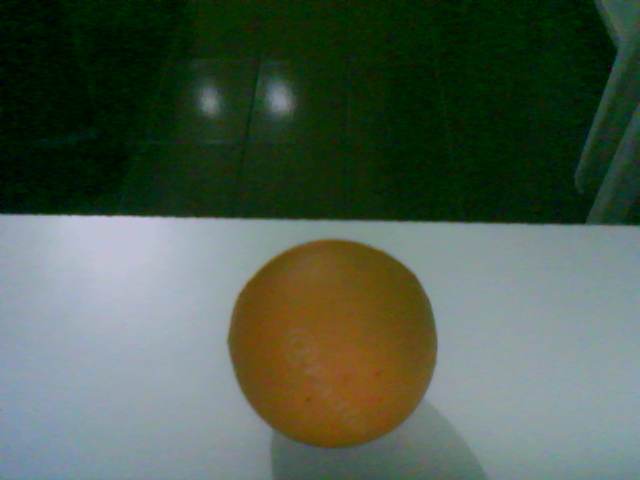
\includegraphics[scale=0.25]{figuras/cam_opencv}}
    \caption{Vídeo sendo reproduzido utilizando a biblioteca OpenCV.}
    \label{img:cam_opencv}
\end{figure}

Outra necessidade importante da aplicação desenvolvida refere-se a interação com o usuário, de modo a permitir que o mesmo seja capaz de selecionar no vídeo reproduzido pela câmera o objeto desejado para detecção e rastreamento. Para possibilitar esse recurso, desenvolveu-se uma funcionalidade onde, ao clicar com um dos botões do mouse no vídeo, a aplicação seja capaz de distinguir o objeto a ser detectado e rastreado.

A aplicação desenvolvida é composta por quatro classes, relacionadas de forma a separar a responsabilidade de cada uma delas, a fim de facilitar o entendimento do código. Esse relacionamento pode ser visto na Figura \ref{rel_sistema}.

\begin{figure}[H]
    \centering
    {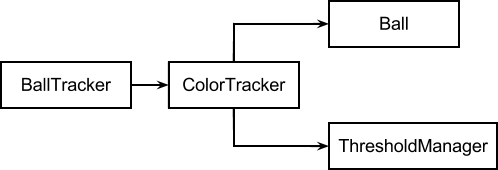
\includegraphics[scale=0.75]{figuras/rel_sistema}}
    \caption{Relacionamento entre as classes do sistema de rastreamento.}
    \label{rel_sistema}
\end{figure}

O Código \ref{code:main_sistema} mostra a inicialização do sistema. Na primeira linha de sua execução, é criado um dicionário com algumas informações pertinentes da janela, sendo elas: nome, largura e altura. Em seguida, um método do OpenCV é usado para nomear a janela a ser criada, utilizando a chave do dicionário que contém o nome desta janela. É instanciado então um vídeo, através do método do OpenCV, passando como parâmetro seu identificador.

Outras instruções no código são relacionadas a lógica para a realização do rastreamento. A criação do objeto \textit{ball\_tracker} (linha 5) tem como responsabilidade a descoberta das coordenadas do círculo, utilizando os valores do objeto a ser detectado e rastreado obtidos pelo clique do mouse. Realizada essa lógica, o objetivo final do objeto \textit{ball\_tracker} é retornar uma instância da classe \textit{Ball} (linha 10), que será utilizada pelo método \textit{circle()} do OpenCV para destacar o objeto no vídeo (linha 12 e 13). Na linha 6, é utilizado outro método da biblioteca, que gerencia os eventos do mouse na tela. Uma repetição, então, é criada com o objeto do vídeo, de forma a obter seus \textit{frames} (linha 7).

Essa implementação permite que, dentro dessa repetição, cada \textit{frame} do vídeo seja capturado e manipulado. O \textit{frame} então é recuperado (linha 8), e, caso seja válido, é usado por outros métodos. No último bloco, é feita a recuperação do objeto \textit{Ball}, contendo as coordenadas necessárias para que um círculo seja desenhado na tela. Esse objeto, então, é usado pelo método do OpenCV que circula a esfera encontrada com uma linha a sua volta e um ponto no meio, todos em azul. Por fim, o \textit{frame} desenhado é inserido na janela criada, de forma a ser visto a partir da interface com o usuário (linha 14).

\begin{code}{python}{Chamada principal do aplicativo.}{code:main_sistema}
if __name__ == '__main__':
	WINDOW_PROPERTIES = {'name': 'Visualisation', 'width': 640, 'height': 480}
	cv2.namedWindow(WINDOW_PROPERTIES['name'])
	video = cv2.VideoCapture(0)
	ball_tracker = BallTracker(video)
	cv2.setMouseCallback(WINDOW_PROPERTIES['name'], on_mouse, [ball_tracker])
	while video.grab():
		flag, frame = video.retrieve()
		if flag:
			ball = ball_tracker.get_ball(frame)
			if ball is not None:
				cv2.circle(frame, (ball.x,ball.y), ball.radius, \
					(255,0,0), 3)
				cv2.circle(frame, (ball.x,ball.y), 3, (255,0,0), -1)
			cv2.imshow(WINDOW_PROPERTIES['name'], frame)
			cv2.waitKey(1)
\end{code}

A classe \textit{BallTracker}, utilizada na chamada principal, está contida no arquivo \textit{tracker.py}, que também possui a classe \textit{ColorTracker}. A primeira, utiliza a segunda para a recuperação do objeto no vídeo baseando-se nos valores HSV do \textit{frame}.

Como ponto de partida, tem-se a chamada do método \textit{get\_ball()}, da classe \textit{BallTracker}, realizada na repetição criada pelo objeto do vídeo (Código \ref{code:get_ball}). Através desse método, é passado para a classe \textit{ColorTracker} o \textit{frame} atual do vídeo, utilizando a  função \textit{find\_ball()}. O espaço de cores desse \textit{frame} é convertido para valores HSV (Figura \ref{img:cam_hsv}) e é devidamente binarizado (Figura \ref{img:cam_bin}). Como pode ser visto no Código \ref{code:find_ball}, que contém a lógica do método \textit{find\_ball()}, são aplicados alguns filtros para melhor detecção dos contornos (linha 5). Após realizados esses tratamentos no \textit{frame}, os contornos são obtidos e utilizados para a recuperação dos parâmetros que compõem o círculo, sendo esses o centróide e raio (linha 6).\newline

\begin{code}{python}{Chamada do método da classe \textit{BallTracker} que recupera os valores do círculo baseando-se pelo \textit{frame} atual.}{code:get_ball}
def get_ball(self, frame):
	return self.color_tracker.find_ball(frame)
\end{code}

\begin{figure}[H]
	\centering
	\subfigure[\textit{Frame} do vídeo em espaço de cor HSV.]{
		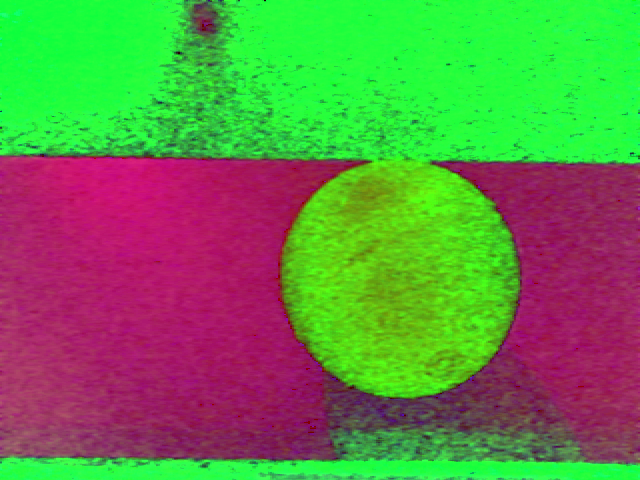
\includegraphics[scale=0.25]{figuras/cam_hsv}
		\label{img:cam_hsv}
	}\hspace{3em}
	\subfigure[\textit{Frame} após aplicação da técnica de binarização.]{
		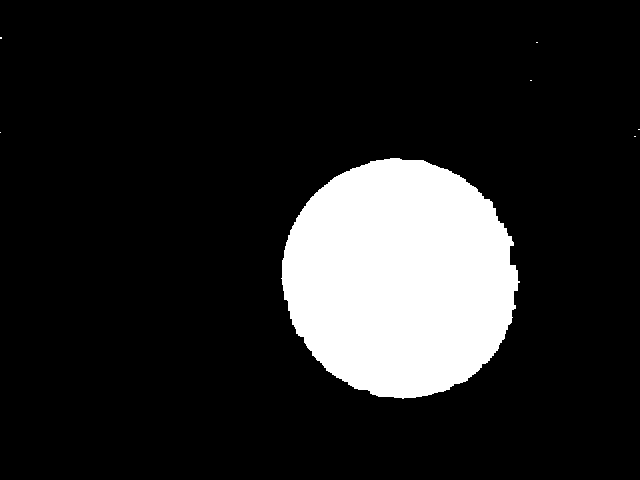
\includegraphics[scale=0.25]{figuras/cam_bin}
		\label{img:cam_bin}
	}
	\caption{Tratamento nos \textit{frames} do vídeo.}
	\label{img:convert_frames}
\end{figure}

\begin{code}{python}{Lógica do método \textit{find\_ball()} da classe \textit{ColorTracker}.}{code:find_ball}
def find_ball(self, frame):
	if self.manager is not None:
		hsv_frame = cv2.cvtColor(frame, cv2.COLOR_BGR2HSV)
		self.thresholded_frame = self.manager.threshold_frame(hsv_frame)
		self.thresholded_frame = self.apply_filters(self.thresholded_frame)
		return self.get_ball(self.thresholded_frame)

def get_ball(self, thresholded):
	contours, hierarchy = cv2.findContours(thresholded, cv2.RETR_TREE, \
		cv2.CHAIN_APPROX_SIMPLE)
	x, y, radius = self.get_ball_parameters(contours)
	ball = Ball(x, y, radius)
	return ball
\end{code}

Como pode ser visto no Código \ref{code:get_ball_parameters}, para a recuperação dos parâmetros do centróide e raio do círculo, é chamada a função que recupera os momentos do contorno da imagem binarizada (linha 6). Recuperado o momento do contorno, uma condição é feita para que sejam buscados os parâmetros apenas dos círculos com área maior que 1000 (linha 8). Dessa forma, evita-se que áreas do vídeo com valores HSV parecidos com o objeto desejado para detecção sejam desenhados, alcançando assim resultados mais próximos do esperado pelo usuário ao clicar com o mouse no vídeo.\newline

\begin{code}{python}{Recuperação dos valores pertinentes para identificar um círculo no \textit{frame} de vídeo.}{code:get_ball_parameters}
def get_ball_parameters(self, contours):
	(...)
	SMALLEST_OBJECT = 1000
	for contour in contours:
		try:
			moments = cv2.moments(contour)
			area = moments['m00']
			if area > SMALLEST_OBJECT:
				x = moments['m10']/area
				y = moments['m01']/area
				radius = sqrt(area/3.14)
		except:
			pass
	return x, y, radius
\end{code}

Para gerenciar o processo de binarização dos \textit{frames}, implementou-se a classe \textit{ThresholdManager}, tornando possível tratar os parâmetros do círculo e aplicá-los quando necessário. Essa classe possui em sua implementação diversas condições de mudança dos valores HSV, para que se ajustem não só a nova condição informada pelo mouse, mas também levando em conta o ambiente.

Quanto aos eventos do mouse, o OpenCV os trata através do método \textit{setMouseCallback()}, como visto anteriormente no Código \ref{code:main_sistema}, responsável por declarar um método que é chamado a cada vez que um evento do mouse é disparado. Este método deve possuir a assinatura especificada pela documentação do OpenCV, contendo o evento a ser disparado, as coordenadas x e y do mouse no vídeo, e um vetor para recuperação dos parâmetros passados pelo método \textit{setMouseCallback()}. Como pode ser visto no Código \ref{code:on_mouse},  esse valores são usados para que, ao clicar com o botão esquerdo do mouse no vídeo, os parâmetros x e y sejam passados para o método \textit{set\_hsv\_values()}. O Código \ref{code:sethsvvalues} mostra a lógica desse método, que converte o \textit{frame} do vídeo atual para o espaço de cor HSV, e através do \textit{frame} convertido, recupera o valor HSV do \textit{pixel} referente as coordenadas x e y passadas como parâmetro para o método.

\begin{code}{python}{Método que recupera informações do clique esquerdo do mouse.}{code:on_mouse}
def on_mouse(event, x, y, flag, param):
	ball_tracker = param[0]
	if event == cv2.EVENT_FLAG_LBUTTON:
		ball_tracker.set_hsv_values(x, y)
\end{code}

\begin{figure}[H]
\end{figure}

\begin{code}{python}{Converte o \textit{frame} para espaço HSV.}{code:sethsvvalues}
def set_hsv_values(self, x, y):
	flag, frame = self.video.retrieve()
	if flag:
		hsv_frame = cv2.cvtColor(frame, cv2.COLOR_BGR2HSV)
		self.color_tracker.new_value(hsv_frame[y][x][0], hsv_frame[y][x][1], \
			hsv_frame[y][x][2])
\end{code}

Dessa forma, os novos valores HSV são passados para o método \textit{new\_value()} da classe \textit{ColorTracker} (Código \ref{code:newvalue}). Em seguida, o método \textit{new\_value()} invoca a classe \textit{ThresholdManager} para que gerencie os novos valores do \textit{pixel}, e inclua-os na binarização dos próximos \textit{frames} do vídeo.

\begin{code}{python}{Um objeto do tipo \textit{ThresholdManager} é instanciado para que trate os valores HSV recuperados através do \textit{pixel} do \textit{frame}.}{code:newvalue}
def new_value(self, h, s, v):
	if self.manager is not None:
		self.manager.add_values(h, s, v)
	else:
		self.manager = ThresholdManager(h, s, v)
\end{code}

A chamada da classe \textit{ThresholdManager} é feita em dois momentos da execução do aplicativo. Na primeira vez em que a ação do clique com o mouse é realizada pelo usuário, o objeto é instanciado passando os valores HSV. Esses valores são então inicializados para criação de dois limiares, contendo valores HSV mínimos e máximos, que serão utilizados para a binarização dos \textit{frames} (Código \ref{code:init_threshold_manager}). Para os próximos eventos disparados pelo mouse, ao invés de instanciar novamente um novo objeto do tipo \textit{ThresholdManager}, o método \textit{add\_values()} é invocado pelo objeto anteriormente criado (Código \ref{code:add_values}).

\begin{code}{python}{Inicialização da classe \textit{ThresholdManager}.}{code:init_threshold_manager}
def __init__(self, h, s, v):
	self.min_h = max(0, h-1)
	self.max_h = min(179, h+1)
	self.min_s = max(0, s-1)
	self.max_s = min(255, s+1)
	self.min_v = 0
	self.max_v = 220
\end{code}

\begin{figure}[H]
\end{figure}

\begin{code}{python}{Método responsável por ajustar os valores HSV do limiares usadas para binarizar o \textit{frame} do vídeo.}{code:add_values}
def add_values(self, h, s, v):
	HUE_MARGIN = 40
	if h < (self.min_h - HUE_MARGIN):
		self.min_h -= 180
		self.max_h -= 180
	elif h > (self.max_h + HUE_MARGIN):
        h -= 180

	if h < self.min_h:
		self.min_h = h-1
	if h > self.max_h:
		self.max_h = min(179, h+1)
	if s < self.min_s:
		self.min_s = max(0, s-1)
	if s > self.max_s:
		self.max_s = min(255, s+1)
\end{code}

Através dessa estrutura lógica, ao clicar com o mouse no objeto desejado para detecção, o mesmo é contornado por um círculo azul e marcado com um ponto, indicando seu centróide. Devido as variações das cores do objeto a ser detectado, causadas pela luminosidade do local, procura-se escolher áreas do objeto contendo cores mais homogêneas. Dessa forma, resultados mais precisos são alcançados, como visto na Figura \ref{img:cam_final}.

\begin{figure}[H]
    \centering
    {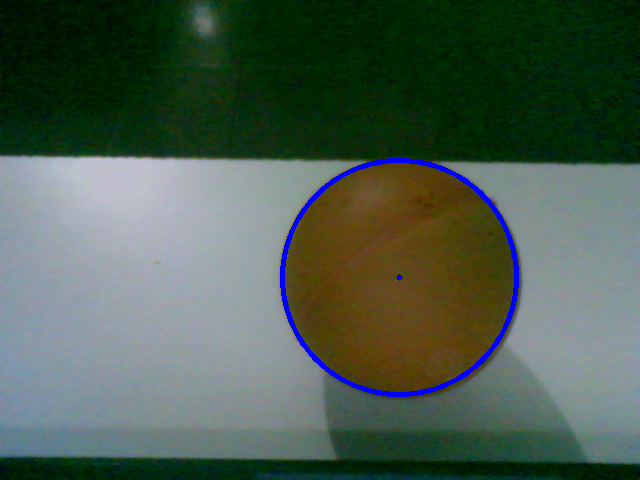
\includegraphics[scale=0.25]{figuras/cam_final}}
    \caption{Resultado final do sistema, detectando uma bola laranja na tela e circulando-a.}
    \label{img:cam_final}
\end{figure}

\section{Resultados}

Como modelo de objeto para detecção e rastreamento, utilizou-se uma bola laranja. Esse objeto foi utilizado em dois planos de fundo, um monocromático e outro policromático. Nesses dois casos, situações foram testadas com o objeto parado e em movimento na cena.

Em um plano de fundo básico, os ajustes dos limiares puderam ser feitos baseando-se em diferentes contrastes de cores referentes ao objeto. Dessa forma, a detecção se mostrou precisa, como mostra a Figura \ref{img:res_basico_parado}, estando o objeto completamente parado. Expondo o mesmo objeto em diferentes velocidades de movimentação no vídeo, os resultados mostraram-se satisfátorios (Figura \ref{img:res_basico_mov}). Em casos onde o objeto se desloca lentamente, o círculo que denota a detecção não possuiu a mesma precisão, porém apresentou um raio de dimensão próxima a original (Figura \ref{img:res_basico_mov1}) (Figura \ref{img:res_basico_mov2}). Nos casos onde o objeto se desloca mais rapidamente, a tendência é que a detecção seja feita acompanhando a tragetória do objeto, porém com precisão menor, fazendo com que o círculo representativo da detecção diminua (Figura \ref{img:res_basico_mov3}).

\begin{figure}[H]
    \centering
    {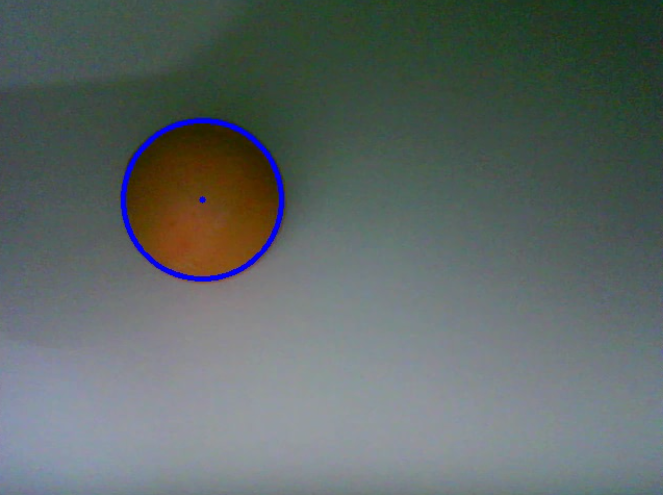
\includegraphics[scale=0.25]{figuras/res_basico1}}
    \caption{Caso básico de detecção, com o objeto parado no vídeo.}
    \label{img:res_basico_parado}
\end{figure}

\begin{figure}[H]
	\centering
	\subfigure[Detecção com pouco deslocamento do objeto.]{
		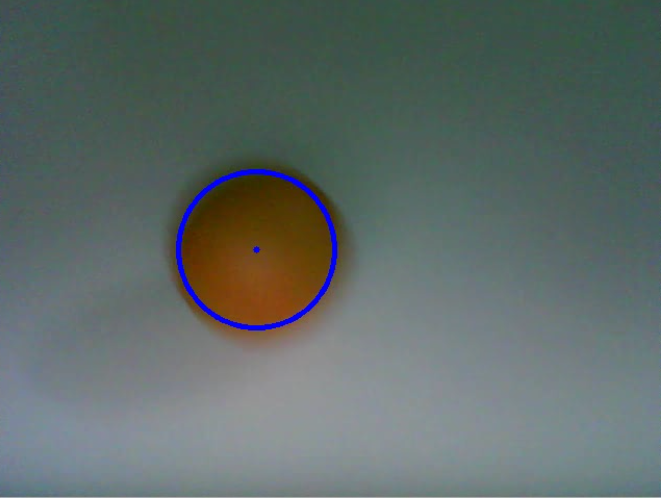
\includegraphics[scale=0.25]{figuras/res_basico_mov1}
		\label{img:res_basico_mov1}
	}\hspace{3em}
	\subfigure[Detecção com médio deslocamento do objeto.]{
		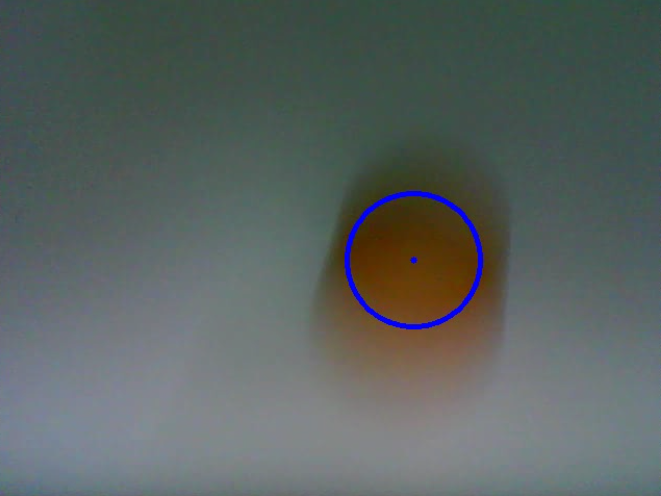
\includegraphics[scale=0.25]{figuras/res_basico_mov2}
		\label{img:res_basico_mov2}
	}\hspace{3em}
	\subfigure[Detecção com muito deslocamento do objeto.]{
		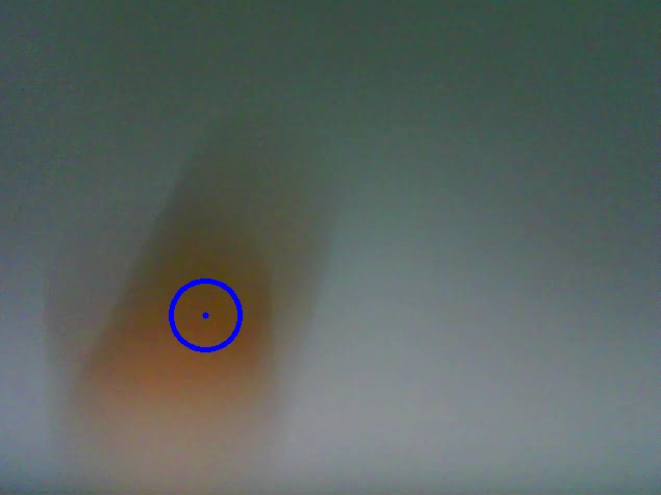
\includegraphics[scale=0.25]{figuras/res_basico_mov3}
		\label{img:res_basico_mov3}
	}
	\caption{Diversos testes feitos com o objeto em diferentes velocidades.}
	\label{img:res_basico_mov}
\end{figure}

Nos casos em que foi utilizado um plano de fundo policromático, a detecção se manteve precisa. Ajustando os limiares com base no novo plano de fundo, o objeto foi rastreado, porém com intermitências em sua detecção. A Figura \ref{img:res_complexo} apresenta casos em que o objeto foi exposto em diferentes distâncias em relação ao vídeo, estando em movimento. Apesar do objeto se apresentar em contraste parecido com o fundo, a aplicação mostrou qualidade na precisão, separando o objeto do plano de fundo complexo.

\begin{figure}[H]
	\centering
	\subfigure[Detecção com o objeto parado em um plano de fundo complexo.]{
		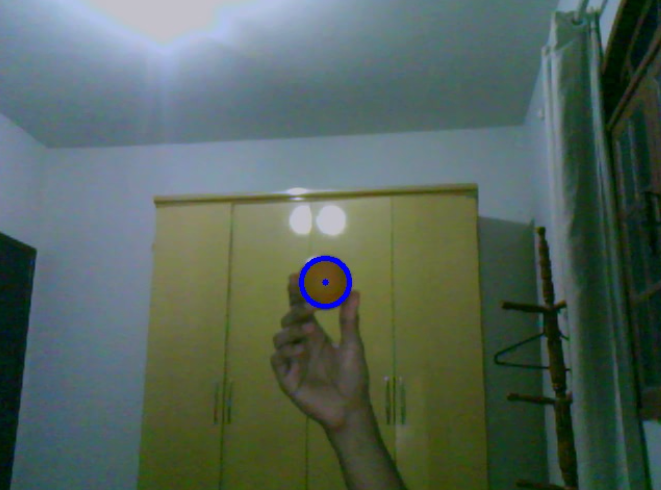
\includegraphics[scale=0.25]{figuras/res_complexo1}
		\label{img:res_complexo1}
	}\hspace{3em}
	\subfigure[Detecção com o objeto em movimento próximo ao vídeo.]{
		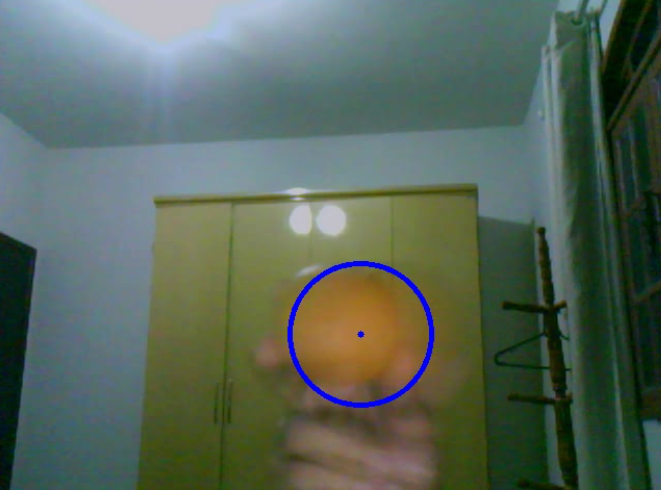
\includegraphics[scale=0.25]{figuras/res_complexo_mov1}
		\label{img:res_complexo_mov1}
	}\hspace{3em}
	\subfigure[Detecção com o objeto em movimento afastado do vídeo.]{
		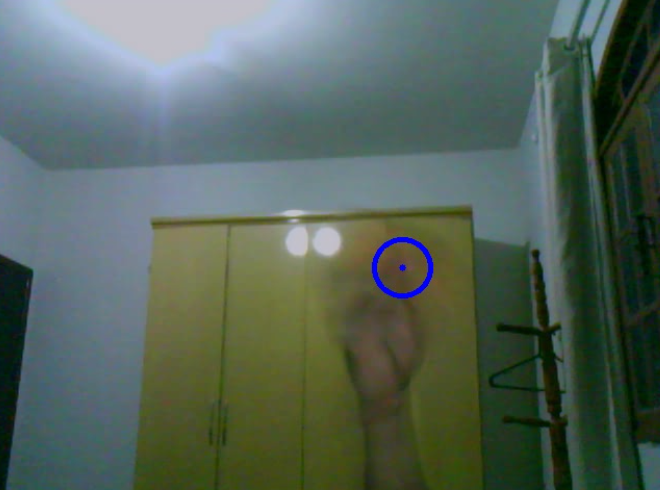
\includegraphics[scale=0.25]{figuras/res_complexo_mov2}
		\label{img:res_complexo_mov2}
	}\hspace{3em}
	\subfigure[Detecção com o objeto em distância média do vídeo.]{
		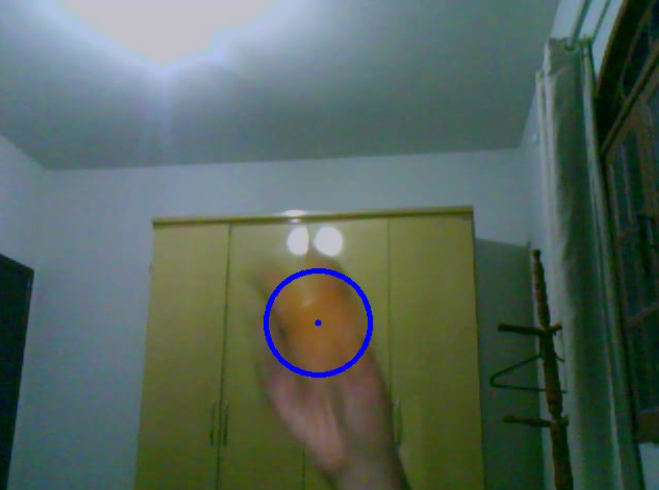
\includegraphics[scale=0.25]{figuras/res_complexo_mov3}
		\label{img:res_complexo_mov3}
	}
	\caption{Diversos testes feitos com o objeto em um plano de fundo complexo, em diferentes proximidades com o vídeo.}
	\label{img:res_complexo}
\end{figure}

No entanto, em alguns casos com o objeto sendo deslocado rapidamente, a detecção não foi feita, assim como nos casos testados com plano de fundo básico (Figura \ref{img:res_complexo_fail}). Apesar de não terem sido realizados testes mais aprofundados, a utilização de equipamentos mais sofisticados para a captura do vídeo e processamento da aplicação podem ocasionar em resultados mais satisfatórios na detecção do objeto.

\begin{figure}[H]
    \centering
    {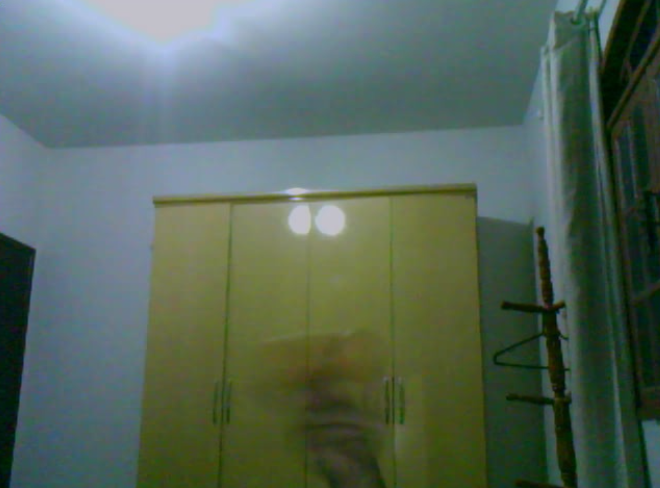
\includegraphics[scale=0.25]{figuras/res_complexo_fail}}
    \caption{Em alguns momentos, a aplicação falhou em detectar o objeto desejado.}
    \label{img:res_complexo_fail}
\end{figure}

Outros casos ainda foram testados considerando outros fatores como iluminação e o objeto não sendo mostrado por completo no vídeo. Os casos em que o objeto é colocado próximo a luz, a aplicação passou a não detectá-lo (Figura \ref{img:res_complexo_luz}). Por terem sido utilizados limiares com base nos tons laranja do objeto, ao aproximá-lo da luz, o tom de cor do mesmo é alterado. Nesses casos, para a correta detecção, é necessário reajustar os limiares de modo a considerar esses novos tons de cores do objeto próximos a luz. Contudo, ao realizar esses ajustes, corre-se o risco da aplicação considerar outros objetos na cena, por possuírem o mesmo tom de cor do objeto.

\begin{figure}[H]
    \centering
    {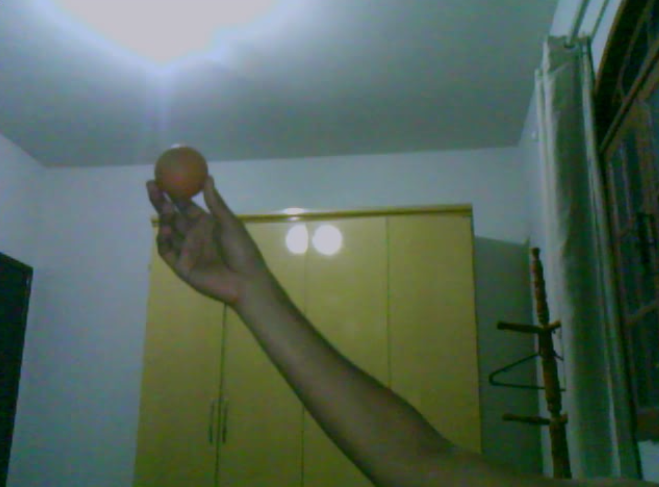
\includegraphics[scale=0.25]{figuras/res_complexo_luz}}
    \caption{Aproximando o objeto da luz artificial, a tendência é que a detecção também falhe.}
    \label{img:res_complexo_luz}
\end{figure}

Nas situações onde o objeto foi apresentado parcialmente no vídeo, os resultados foram positivos. A Figura \ref{img:res_complexo_obst} apresenta alguns casos onde o objeto foi apresentado com alguns obstáculos.

\begin{figure}[H]
	\centering
	\subfigure[Caso em que detecção foi bem sucedida mesmo sendo mostrada parcialmente no vídeo.]{
		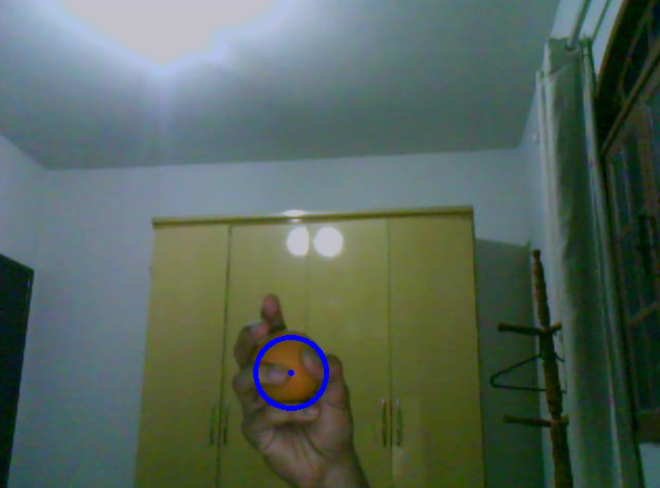
\includegraphics[scale=0.25]{figuras/res_complexo_obst1}
		\label{img:res_complexo_obst1}
	}\hspace{3em}
	\subfigure[Segundo caso onde o resultado foi positivo para detecção com obstáculos.]{
		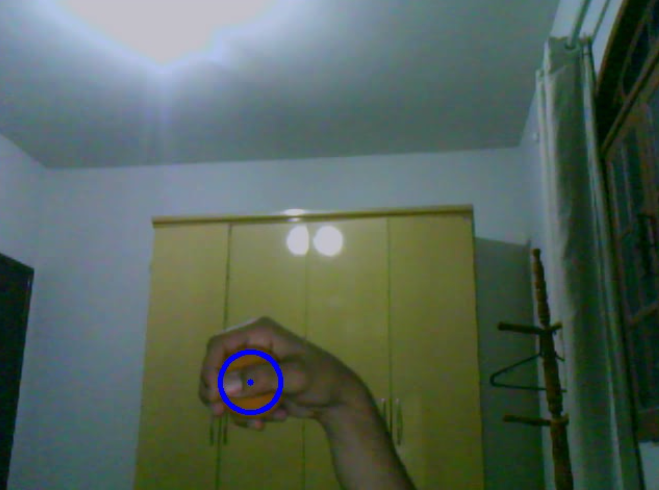
\includegraphics[scale=0.25]{figuras/res_complexo_obst2}
		\label{img:res_complexo_obst2}
	}
	\caption{Casos de sucesso na detecção do objeto em situações adversas.}
	\label{img:res_complexo_obst}
\end{figure}
